\documentclass[10pt]{beamer}

%\usepackage[backend=bibtex,firstinits=true,style=verbose-inote,citestyle=authortitle]{biblatex}
\usepackage{bm}
\usepackage{graphicx}
\usepackage{subcaption}
\usepackage{amsmath}
\usepackage{amsfonts}
\usepackage{makecell}
\usepackage{filecontents}
\usepackage{biblatex}
\usepackage{listings}
\usepackage{xcolor}
%\usepackage{systeme}
%\usepackage[english]{babel}
\usepackage[utf8]{inputenc}
\usepackage{fancyhdr}
\usepackage{amsmath,amssymb,amsfonts,amsthm}
\usepackage{indentfirst}
\usepackage{bm}
\usepackage[a4paper, total={6in, 10in}]{geometry}

% For using subfigures
\usepackage{graphicx}
\usepackage{caption}
\usepackage{subcaption}

% To put a figure where it is
\usepackage{float}

\usepackage{tensor}
\usepackage{biblatex}
\usepackage{titlesec}
\usepackage{bbm, dsfont} % For indicator functions
\usepackage{mathtools} % for \coloneqq
\usepackage[bottom]{footmisc} % prevents pictures going below footnote :|
% \usepackage{pifont} % for \ding{...}

\addbibresource{../../articles/articles.bib}

% \newcommand\defeq{\stackrel{\mathclap{\normalfont\mbox{def}}}{=}}

\newcommand{\expect}[2][]{
\ifthenelse{\equal{#1}{}}{
\mathbb{E}\left[#2\right]
}{
\underset{#1}{\mathbb{E}}\left[#2\right]
}}

\newcommand{\cov}[2][]{
\ifthenelse{\equal{#1}{}}{
\text{Cov}\left[#2\right]
}{
\underset{#1}{\text{Cov}}\left[#2\right]
}}


\newcommand{\var}[2][]{
\ifthenelse{\equal{#1}{}}{
\text{Var}[#2]
}{
\underset{#1}{\text{Var}}[#2]
}}

\newcommand{\loss}[2][]{
\ifthenelse{\equal{#1}{}}{
\mathcal{L}(#2)
}{
\mathcal{L}_{#1}(#2)
}}

\newcommand{\kl}[2]{
\text{D}_\text{KL}[#1 \parallel #2]
}

\newcommand{\R}{\mathbb{R}}
%\newcommand{\Prob}{\mathbb{P}}

\newcommand{\1}[1]{\mathds{1}\{#1\}}

% We need this for \begin{theorem}...\end{theorem} staff
\newtheorem*{theorem*}{Theorem}
\newtheorem{theorem}{Theorem}
\newtheorem*{proposition*}{Proposition}
\newtheorem{proposition}{Proposition}
\newtheorem*{corollary*}{Corollary}
\newtheorem{corollary}{Corollary}
\newtheorem*{lemma*}{Lemma}
\newtheorem{lemma}{Lemma}
\newtheorem*{question*}{Question}
\newtheorem{question}{Question}

\theoremstyle{definition}
\newtheorem{definition}{Definition}[section]


%\usecolortheme{dolphin}
\setbeamertemplate{navigation symbols}{}
\setbeamertemplate{section in toc}{\inserttocsectionnumber.~\inserttocsection}

\begin{filecontents*}{references.bib}
@misc{masks_for_random_nns,
Author = {Vivek Ramanujan and Mitchell Wortsman and Aniruddha Kembhavi and Ali Farhadi and Mohammad Rastegari},
Title = {What's Hidden in a Randomly Weighted Neural Network?},
Year = {2019},
Eprint = {arXiv:1911.13299},
}
\end{filecontents*}

\addbibresource{references.bib}


\title{What’s Hidden in a Randomly Weighted Neural Network? \footnote{\citepaper{masks_for_random_nns}}}
%\subtitle{}
%\author{Ivan Skorokhodov}
%\date{}
%\logo{
\includegraphics[height=1cm]{images/ipavlov-logo.png}}

\newcommand{\citepaper}[1]{\citetitle{#1} by \citeauthor{#1}}

%\graphicspath{{./images}}

%\usetheme{lucid}
\begin{document}

\begin{frame}
    \titlepage
\end{frame}

\begin{frame}{Overview}
    \begin{itemize}
        \item\pause Authors took a randomly initialized model.
        \item\pause Then they trained a binary mask for this model to extract a good subnetwork.
        \item\pause The performance of this subnetwork turned out to be very good.
    \end{itemize}
    
    \pause
    \begin{figure}
        \centering
        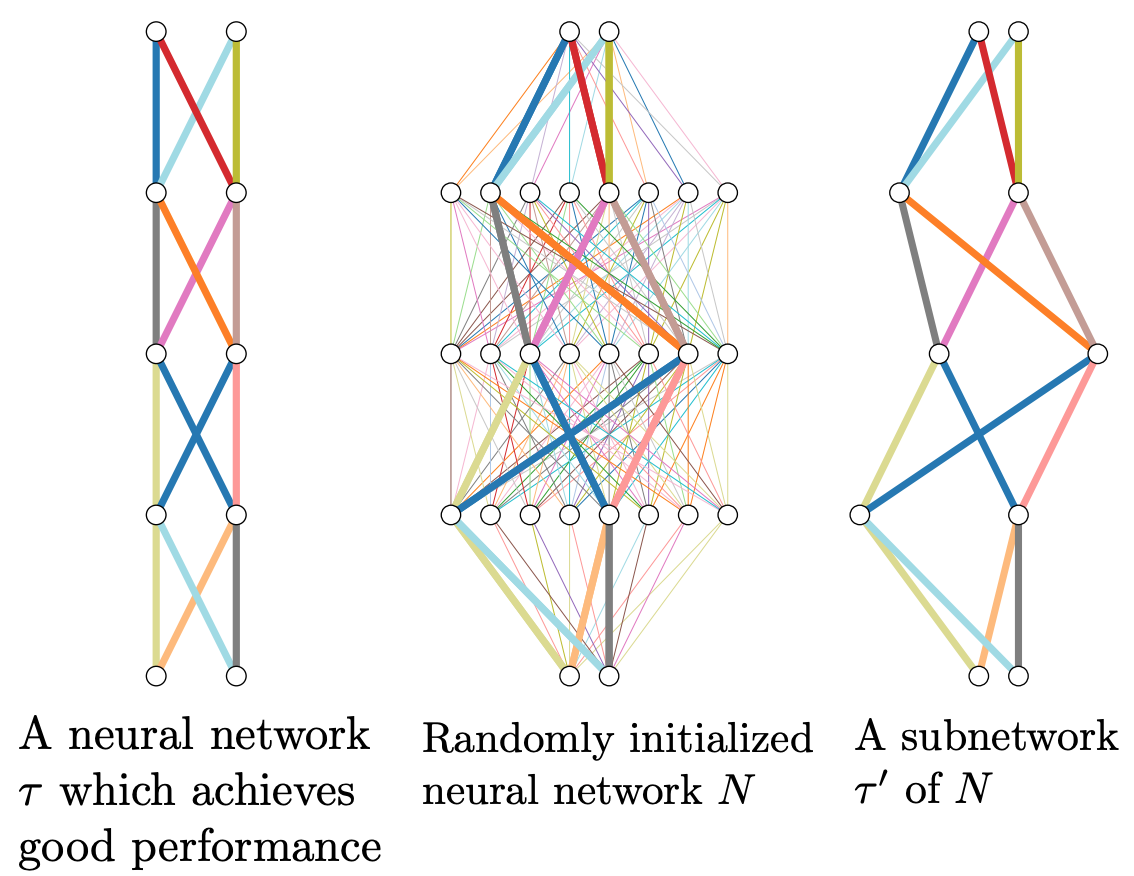
\includegraphics[width=0.5\textwidth]{images/illustration.png}
        \caption{Since we have combinatorial number of subnetworks and modern models have millions of parameters we are likely to find a good one.}
    \end{figure}
\end{frame}

\begin{frame}{How to find a good subnetwork}
\begin{enumerate}
    \item\pause Initialize the model randomly
    \item\pause Associate a score $s_{uv}$ with each synapse $u \to v$.
    \item\pause Use weights that have top $k\%$ scores for forward pass.
    \item\pause Use straight-through estimator (STE) to train the scores.
\end{enumerate}

\pause
Normally, input at neuron $v$ is computed as:
\begin{equation}
\mathcal{I}_{v}=\sum_{(u, v) \in \mathcal{E}} w_{u v} \mathcal{Z}_{u}
\end{equation}

\pause
When we learn scores, we compute it as:
\begin{equation}
\mathcal{I}_{v}=\sum_{u \in \mathcal{V}^{(\ell-1)}} w_{u v} \mathcal{Z}_{u} h\left(s_{u v}\right),
\qquad
h(s_{uv}) = \begin{cases}
        1, \text{if }s_{uv}\text{ is in top-k scores}, \\
        0, \text{otherwise}
    \end{cases}
\end{equation}

\pause
And we update it via STE:
\begin{equation}
\tilde{s}_{u v}=s_{u v}-\alpha \frac{\partial \mathcal{L}}{\partial \mathcal{I}_{v}} w_{u v} \mathcal{Z}_{u}
\end{equation}

\end{frame}


\begin{frame}[fragile]{Straight-through estimator (STE)}
\begin{itemize}
    \item Imagine, we have a non-differentiable function $f(\theta)$
    \begin{itemize}
        \item\pause for example, thresholding 5\% of the highest values
    \end{itemize}
    \item Imagine, we use it in the computation of some complex function $L(f(\theta), x)$.
    \begin{itemize}
        \item\pause for example, classification loss on a batch $x$.
    \end{itemize}
    \item\pause STE is a trick to compute the gradients w.r.t. to $\theta$ through $f$:
    \begin{itemize}
        \item\pause During forward pass, use $f(\theta)$ as is.
        \item\pause During backward pass, replace $f(\theta)$ with just $\theta$!
        \item\pause I.e. we compute the loss using the real value $f(\theta)$, but ``remove'' gradients from chain-rule multiplication that we cannot compute
        \item\pause Imagine that $L(f(\theta), x) = a(f(\theta(s)), x)$, then:
        \begin{equation*}
            \partial_\theta L = \frac{\partial L}{\partial a} \frac{\partial a}{\partial f} \textcolor{red}{\frac{\partial f}{\partial \theta}} \frac{\partial \theta}{\partial s} \approx \frac{\partial L}{\partial a} \frac{\partial a}{\partial f} \frac{\partial \theta}{\partial s}
        \end{equation*}
    \end{itemize}
\end{itemize}

\pause
The best explanation of STE:

\begin{lstlisting}[language=Python]
def straight_through_estimation(x, f):
  # In forward pass it is equal to f(x)
  # In backward pass `(...).detach()` term vanishes
  return (f(x) - x).detach() + x
\end{lstlisting}

%\begin{lstlisting}
%    asdf
%\end{lstlisting}

%\begin{lstlisting}
%// Gestion du contexte ete2013
%// Utilisation d'un nouveau template
%if (%variables['ctpage'] == "ete2013") {
%    variables['template_files']=array('page-ete');
%}
%\end{lstlisting}

\end{frame}


\begin{frame}{Results}
    \pause
    Authors tried two different initializations:
    \begin{itemize}
        \item\pause Kaiming Normal (for ReLU it is $\mathcal{D}_{\ell}=\mathcal{N}(0, \sqrt{2 / n_{\ell-1}})$)
        \item\pause Signed Constant: set each weight to $\sigma$, then randomly choose its $+/-$ sign
    \end{itemize}
    
    \begin{figure}
        \centering
        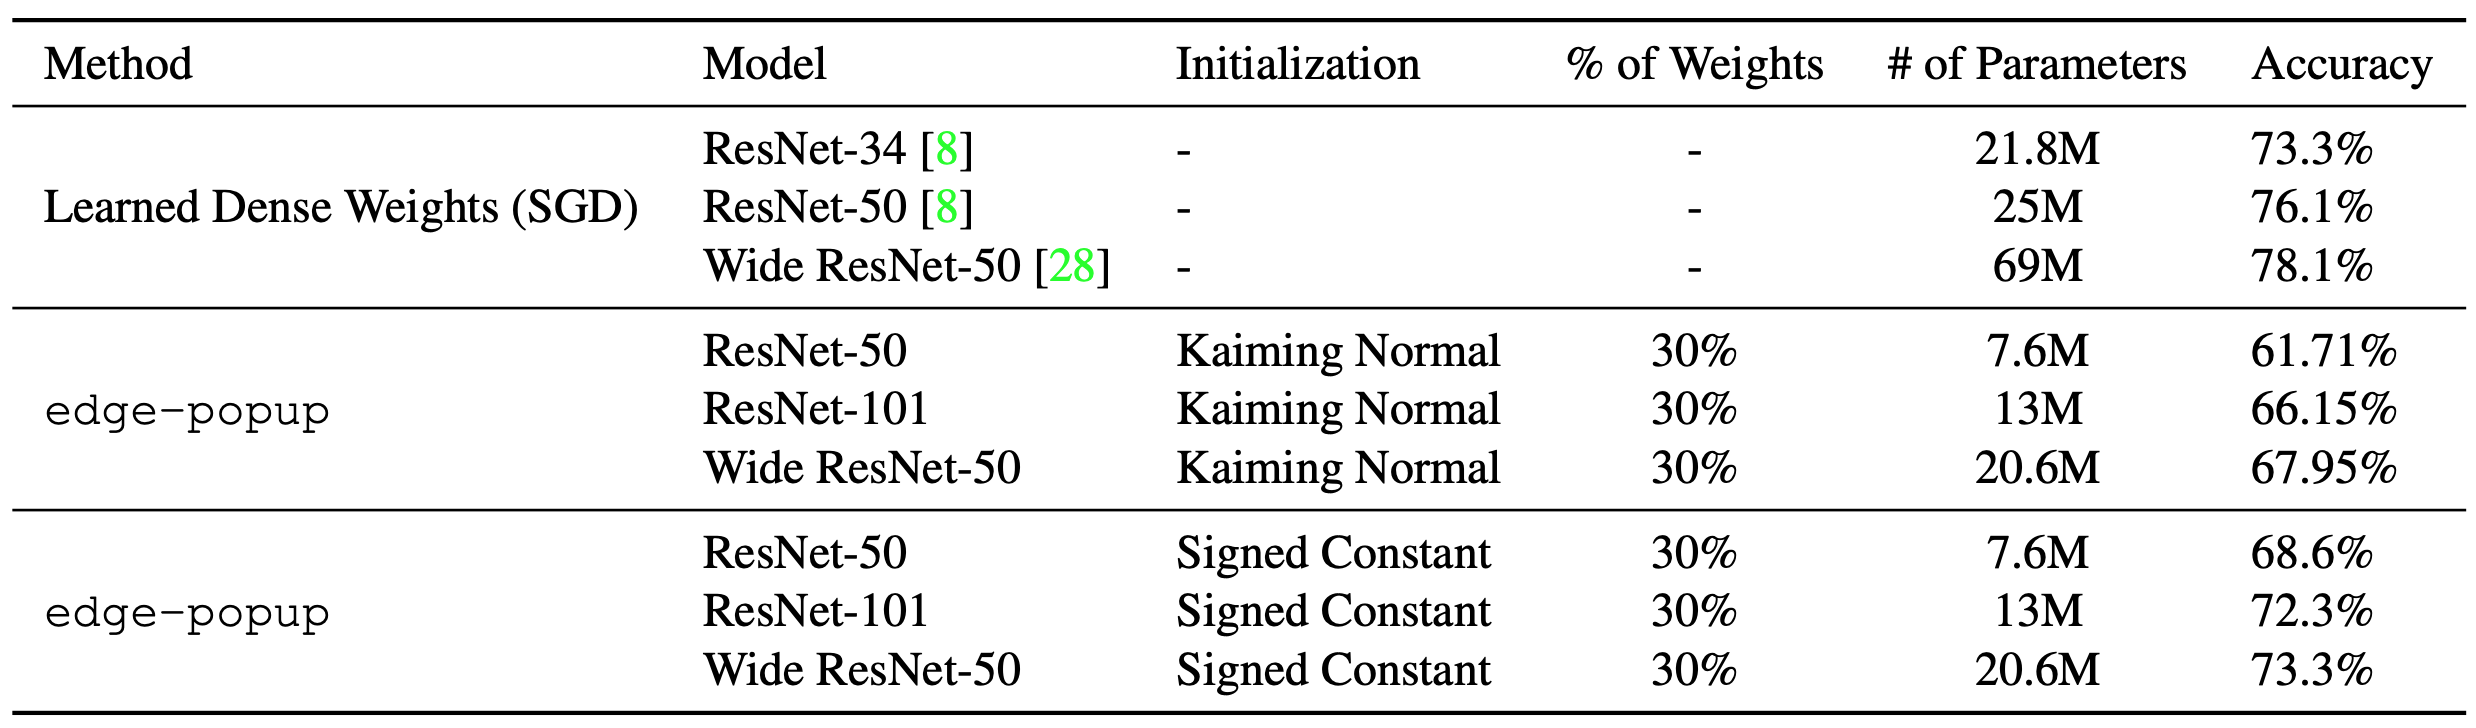
\includegraphics[width=\textwidth]{images/imagenet-results}
        \caption{ImageNet results (with $k=30\%$)}
    \end{figure}
\end{frame}

\begin{frame}{Varying \% of remaining weights}
    \begin{figure}
        \centering
        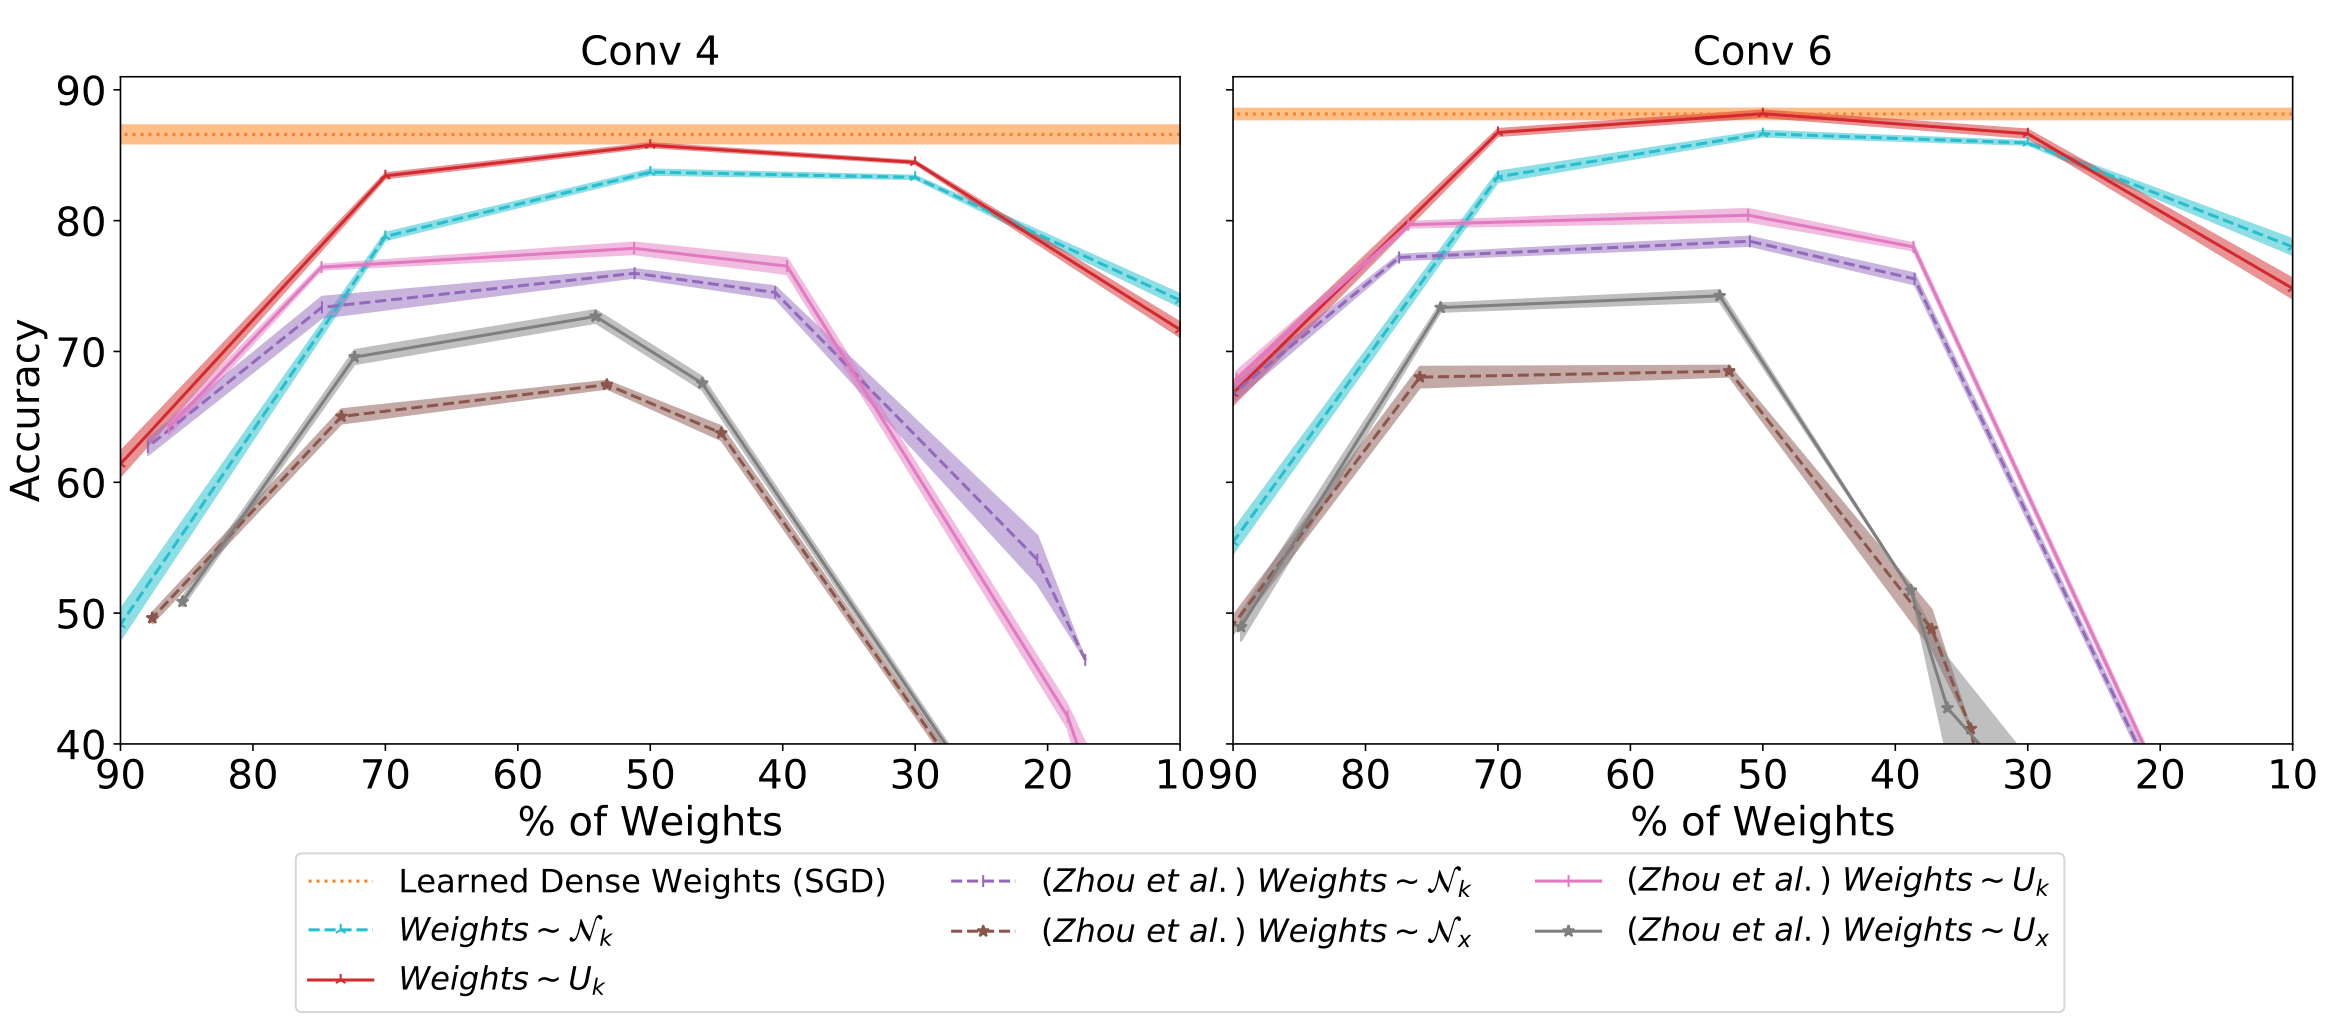
\includegraphics[width=\textwidth]{images/varying-k}
        \caption{Varying \% of remaining weights for AlexNet for CIFAR-10. Maximum in the middle since $\binom{n}{k}$ is maximized at $k \approx n/2$}
    \end{figure}
\end{frame}


\begin{frame}{Varying width of a specific layer}
    \begin{figure}
        \centering
        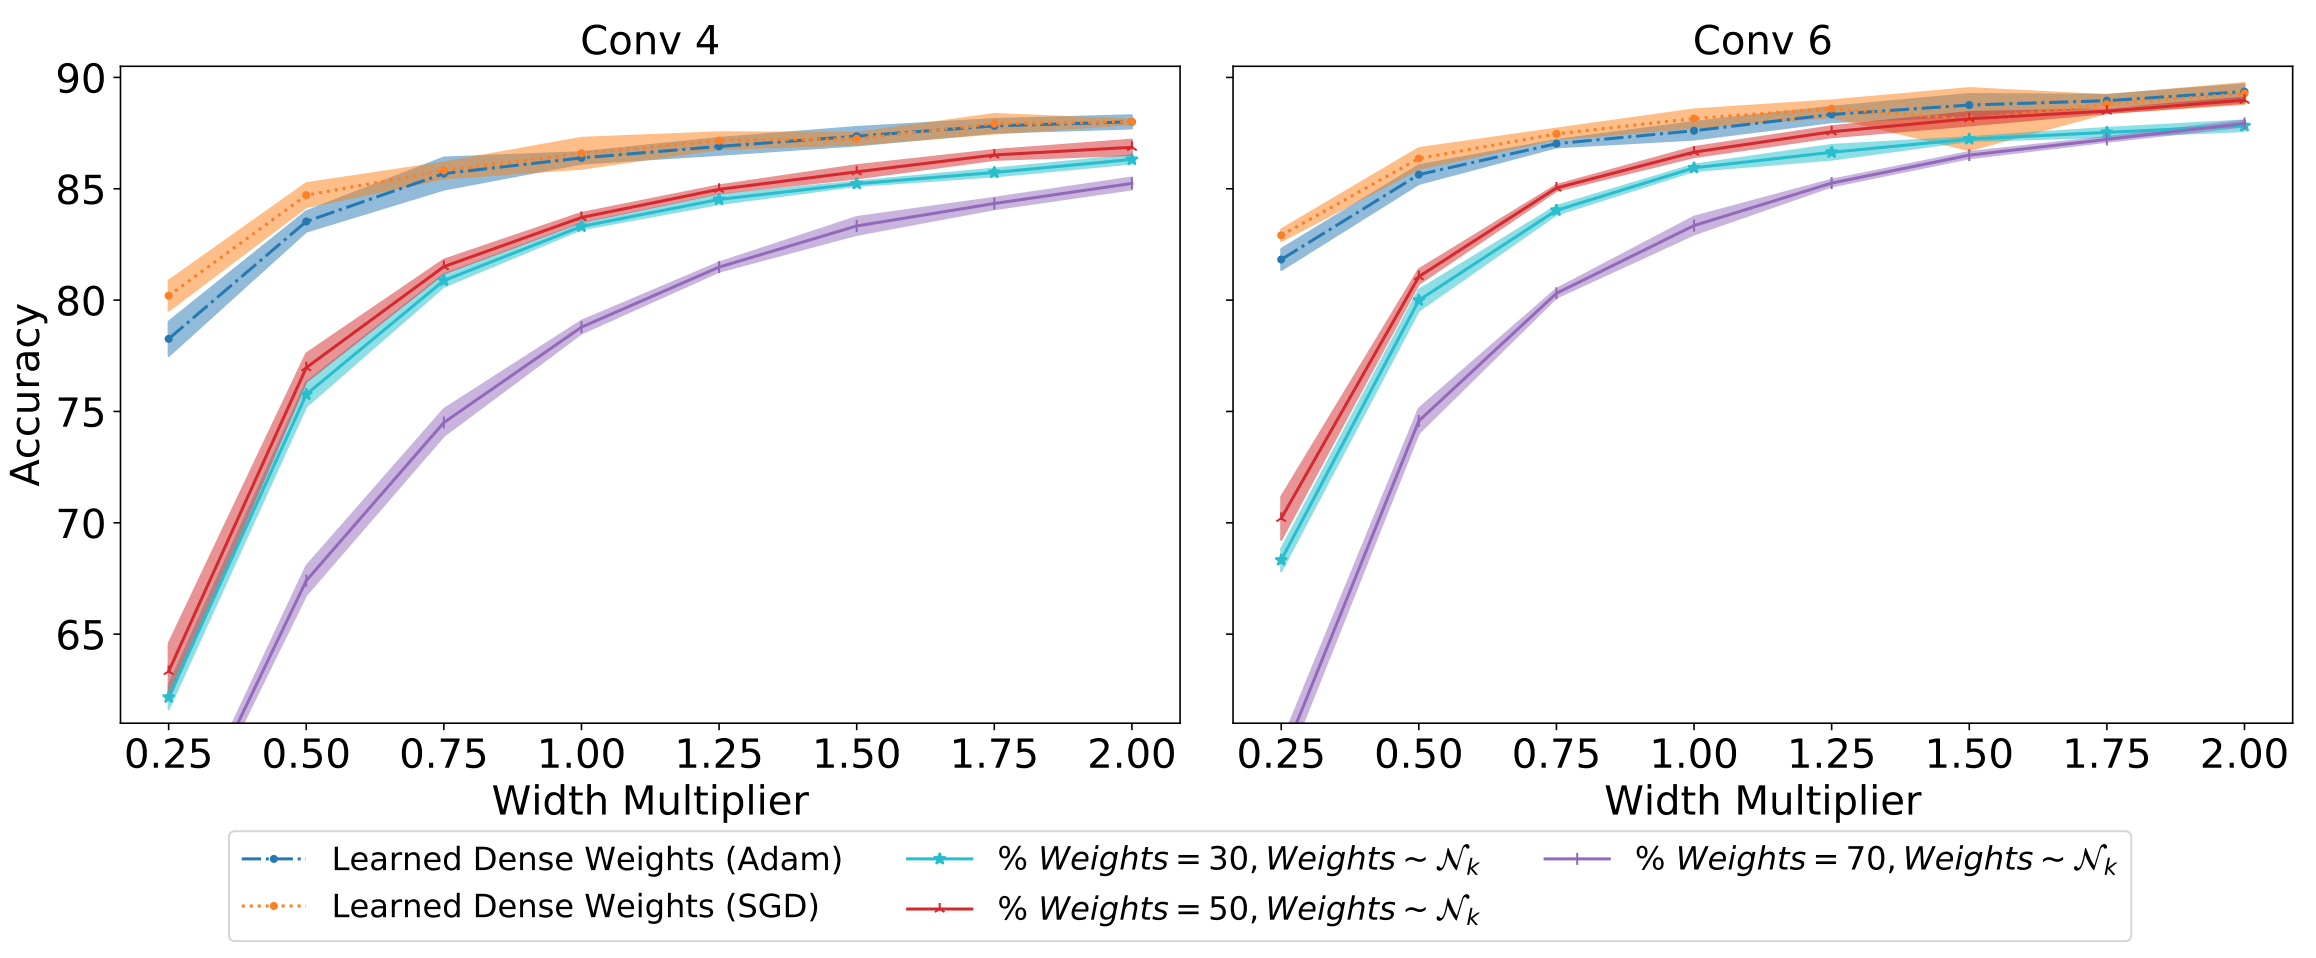
\includegraphics[width=\textwidth]{images/varying-width-alexnet}
        \caption{Varying width of a layer for AlexNet for CIFAR-10}
    \end{figure}
\end{frame}


%\begin{frame}{Scaled vs Unscaled init}
%    Since only $k\%$ of the neurons are ``used'' we would better
%\end{frame}

%\begin{frame}{Scaled vs Unscaled Weight initialization}
%    
%\end{frame}

%\begin{frame}{Results}
%    
%\end{frame}

\begin{frame}{Conclusion}
\begin{itemize}
    \item\pause Random weights with a good connectivity pattern work as good as trained weights.
    \item\pause Signed Constant init works better than Kaiming Normal init, which means that precise weights values are not important. We just need magnitudes and a connectivity pattern.
    \item\pause HAT-algorithm for CL is not ``fair''?
\end{itemize}
\end{frame}

\end{document}
